\documentclass[assignment3.tex]{subfiles}
\begin{document}

\section*{3η Άσκηση}
Παρατηρείται ότι το πολυώνυμο δίνεται σε φωλιασμένη μορφή άρα είναι πολυώνυμο \textlatin{Newton}. Επομένως, μπορεί πολύ εύκολα να υπολογιστεί ένα νέο πολυώνυμο που να παρεμβάλει και το πέμπτο σημείο.

Συγκεκριμένα, αν $p_3=2-(x+1)+x(x+1)-2x(x+1)(x-1)$ τρίτου βαθμού πολυώνυμο, τότε το νέο πολυώνυμο $p_4(x)$ θα είναι της μορφής (\ref{eq:newton_extraterm}) και θα είναι τέταρτου βαθμού. 
\begin{equation}
p_4(x) = p_3(x) + cx(x+1)(x-1)(x-2)
\label{eq:newton_extraterm}
\end{equation}
Ο προσδιορισμός της σταθεράς $c$ γίνεται μέσω της τιμής του νέου πολυωνύμου στο επιπλέον σημείο (\ref{eq:newton_extraterm_constant}). 

Το υπολογιστικό φορτίο που απαιτείται για να προστεθεί ένας επιπλέον όρος είναι μικρό: 8 πράξεις κινητής υποδιαστολής (4 προσθαφαιρέσεις, 3 πολλαπλασιασμοί και 1 διαίρεση). Εδώ φαίνεται η υπεροχή της χρήσης των πολυωνύμων \textlatin{Newton} σε σχέση με τα πολυώνυμα \textlatin{Lagrange}, για τα οποία θα χρειαζόταν ο υπολογισμός όλου του πολυωνύμου εξαρχής.

\begin{equation}
\begin{split}
p_4(x_4) &= 10 \rightarrow \\
 y_4 &= p_3(x_4) + cx_4(x_4+1)(x_4-1)(x_4-2) \rightarrow \\
 c &= \frac{y_4-p_3(x_4)}{x_4(x_4+1)(x_4-1)(x_4-2)}
\end{split}
\label{eq:newton_extraterm_constant}
\end{equation}
Στο Σχήμα \ref{fig:ex3} δίνονται τα $p_3(x)$ και $p_4(x)$. Όπως είναι αναμενόμενο, τα δύο πολυώνυμα είναι σχετικά κοντά μέχρι το $(2,-7)$ και αποκλίνουν σημαντικά μετά από αυτό.

\begin{figure}[hp]
	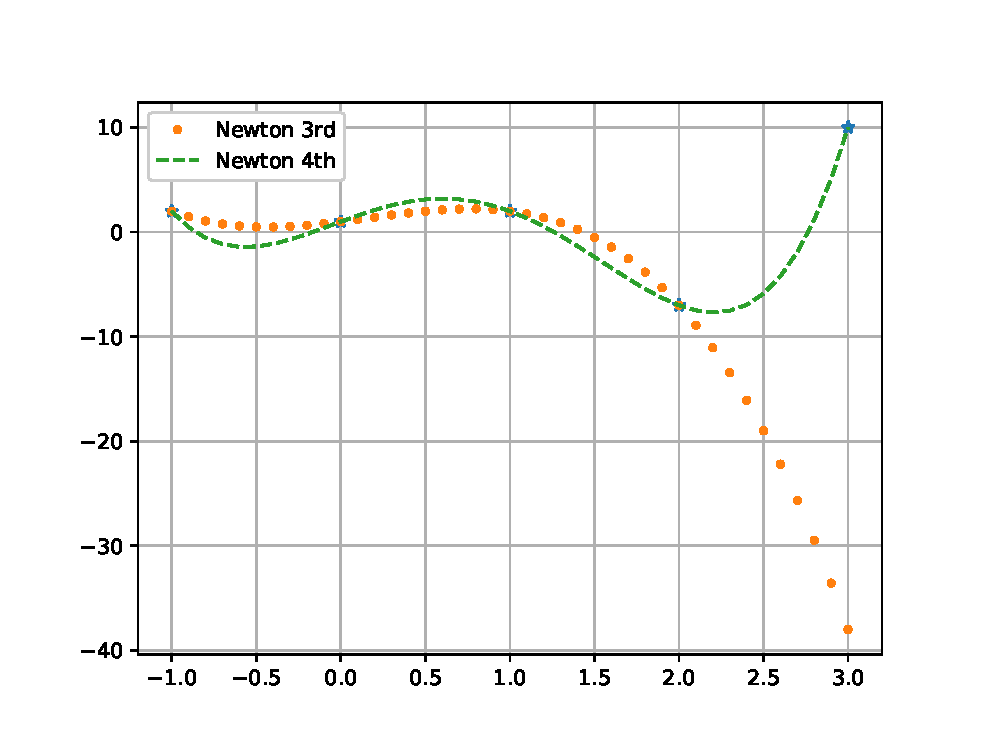
\includegraphics[width=0.9\textwidth]{ex3.eps}
	\centering
	\caption{Παρεμβολή με πολυώνυμα \textlatin{Newton} 3ου και 4ου βαθμού}
	\label{fig:ex3}
\end{figure}

Παρακάτω ακολουθεί ο κώδικας που γράφτηκε σε \textlatin{Python} και έγινε χρήση της βιβλιοθήκης \textlatin{Numpy}. Η υλοποίηση των αλγορίθμων προσθήκης νέου όρου στο πολυώνυμο \textlatin{Newton} και φωλιασμένου υπολογισμού της τιμής του πολυωνύμου δίνονται στο Παράρτημα.
\selectlanguage{english}
\lstinputlisting[style=python, firstline=8]{ex3.py}
\end{document}